%% lbm_paper.tex -- IEEE Journal, HPSC 2026 Assignment
\documentclass[journal]{IEEEtran}

\usepackage{amsmath,amssymb}
\usepackage{graphicx}
\usepackage{booktabs}
\usepackage{array}
\usepackage{multirow}
\usepackage{url}
\usepackage{cite}
\usepackage{xcolor}

\graphicspath{{plots/}}
\DeclareGraphicsExtensions{.png,.pdf}

\hyphenation{op-tical net-works semi-conduc-tor OpenMP}

\begin{document}

\title{Performance Analysis of D2Q9 Lattice Boltzmann\\
       Fluid Simulation Across HPC Backends}

\author{Rahul~Kumar~Rawat%
\thanks{Submitted in partial fulfilment of HPSC 2026.
        April 2026.
        Code: \url{https://github.com/rahulkumar67-del/Hpsc_Assignment}}}

\markboth{HPSC 2026}%
{Rawat: Performance Analysis of D2Q9 LBM Across HPC Backends}

\maketitle

%% =====================================================================
\begin{abstract}
This paper presents the design, implementation, verification, and
performance analysis of a two-dimensional Lattice Boltzmann Method
(LBM) fluid solver using the D2Q9 velocity model with the
Bhatnagar--Gross--Krook (BGK) collision operator.  Two canonical test
cases are studied: the lid-driven cavity and flow past a circular
cylinder.  The solver is implemented in C++17 with three computational
backends --- serial, OpenMP (shared-memory parallelism), and MPI
(message-passing scaffold).  Grid convergence is verified across five
mesh resolutions from $32\times32$ to $512\times512$.  Performance
benchmarks demonstrate that OpenMP parallelisation achieves
near-linear speedup on larger grids: at $p=8$ threads on a
$512\times512$ mesh, the measured speedup exceeds $5\times$ with an
efficiency above 65\%.  The throughput metric MLUPS (Million Lattice
Updates Per Second) confirms that OpenMP consistently outperforms the
serial baseline across all tested grid sizes.  Results are consistent
with Amdahl's Law as the parallelisable fraction of the collision-streaming
loop dominates total runtime.
\end{abstract}

\begin{IEEEkeywords}
Lattice Boltzmann Method, D2Q9, BGK collision, lid-driven cavity,
flow past cylinder, OpenMP, MPI, shared-memory parallelism,
performance scaling, MLUPS.
\end{IEEEkeywords}

\IEEEpeerreviewmaketitle

%% =====================================================================
\section{Introduction}
\IEEEPARstart{T}{he} Lattice Boltzmann Method (LBM) has emerged as a
powerful alternative to conventional Navier--Stokes solvers for
computational fluid dynamics~\cite{chen1998}.  Rather than discretising
the macroscopic conservation equations directly, LBM evolves particle
distribution functions on a regular lattice through local collision
and streaming steps.  This mesoscopic approach offers several
advantages: inherent parallelism due to data locality, straightforward
handling of complex boundary geometries via bounce-back rules, and
natural incorporation of multiphase and multicomponent
physics~\cite{succi2001}.

For two-dimensional incompressible flows at low Mach number, the D2Q9
lattice model with the single-relaxation-time BGK collision
operator~\cite{bgk1954} provides an efficient and well-validated
framework.  The computational cost of LBM scales linearly with the
number of lattice nodes $N$, and the collision step is embarrassingly
parallel --- each node can be updated independently --- making LBM
an ideal candidate for shared-memory parallelisation with
OpenMP~\cite{openmp2018}.

This work addresses the complete scientific-computing workflow:
mathematical formulation of the D2Q9-BGK model (\S\ref{sec:math}),
numerical algorithm design (\S\ref{sec:algo}), software implementation
with multiple HPC backends (\S\ref{sec:impl}), verification through
grid convergence and comparison with established benchmarks
(\S\ref{sec:verify}), and a quantitative performance study across
serial, OpenMP, and MPI backends (\S\ref{sec:perf}).

%% =====================================================================
\section{Mathematical Formulation}
\label{sec:math}

\subsection{The Lattice Boltzmann Equation}
The discrete Boltzmann equation with the BGK collision
operator~\cite{bgk1954} reads:
\begin{equation}
  f_q(\mathbf{x} + \mathbf{c}_q \Delta t,\; t + \Delta t)
  = f_q(\mathbf{x}, t)
  - \omega\bigl[f_q(\mathbf{x}, t) - f_q^{\mathrm{eq}}(\mathbf{x}, t)\bigr],
  \label{eq:lbe}
\end{equation}
where $f_q$ is the particle distribution function for discrete velocity
direction $q$, $\mathbf{c}_q$ is the corresponding lattice velocity
vector, $\omega = 1/(3\nu + \tfrac{1}{2})$ is the relaxation frequency,
and $\nu$ is the kinematic viscosity.

\subsection{D2Q9 Velocity Model}
The D2Q9 model uses nine discrete velocities in two dimensions:
\begin{equation}
  \mathbf{c}_q = \begin{cases}
    (0,0) & q = 0 \\
    (\cos\theta_q, \sin\theta_q) & q = 1{-}4,\; \theta_q = (q{-}1)\pi/2 \\
    \sqrt{2}(\cos\theta_q, \sin\theta_q) & q = 5{-}8,\; \theta_q = (q{-}5)\pi/2 + \pi/4
  \end{cases}
\end{equation}
with lattice weights $w_0 = 4/9$, $w_{1-4} = 1/9$, and
$w_{5-8} = 1/36$.

\subsection{Equilibrium Distribution}
The Maxwell--Boltzmann equilibrium truncated to second order is:
\begin{equation}
  f_q^{\mathrm{eq}} = w_q \rho \left[
    1 + 3(\mathbf{c}_q \cdot \mathbf{u})
    + \tfrac{9}{2}(\mathbf{c}_q \cdot \mathbf{u})^2
    - \tfrac{3}{2}|\mathbf{u}|^2
  \right],
  \label{eq:feq}
\end{equation}
where the macroscopic density and velocity are recovered as:
\begin{equation}
  \rho = \sum_{q=0}^{8} f_q, \qquad
  \rho\mathbf{u} = \sum_{q=0}^{8} f_q \mathbf{c}_q.
  \label{eq:macro}
\end{equation}

\subsection{Viscosity and Reynolds Number}
The kinematic viscosity is related to the relaxation parameter by:
\begin{equation}
  \nu = \frac{1}{3}\left(\frac{1}{\omega} - \frac{1}{2}\right),
  \qquad
  \mathrm{Re} = \frac{u_{\mathrm{lid}} \cdot L}{\nu}.
  \label{eq:re}
\end{equation}

%% =====================================================================
\section{Numerical Algorithm}
\label{sec:algo}

\subsection{Collision--Streaming Decomposition}
Each timestep consists of two phases applied to every interior lattice
node:

\paragraph{Collision} Relax each distribution toward equilibrium:
\begin{equation}
  f_q^{*}(\mathbf{x}, t) = f_q(\mathbf{x}, t)
  - \omega\bigl[f_q(\mathbf{x}, t) - f_q^{\mathrm{eq}}(\rho, \mathbf{u})\bigr].
  \label{eq:collide}
\end{equation}

\paragraph{Streaming} Propagate post-collision distributions to
neighbouring nodes:
\begin{equation}
  f_q(\mathbf{x} + \mathbf{c}_q, t + 1) = f_q^{*}(\mathbf{x}, t).
  \label{eq:stream}
\end{equation}

\subsection{Boundary Conditions}

\paragraph{No-slip walls (bounce-back)}
At solid boundaries and obstacle surfaces, the incoming distribution
is reflected to the opposite direction:
$f_{\bar{q}}(\mathbf{x}_w) = f_q^{*}(\mathbf{x}_w)$,
where $\bar{q}$ denotes the direction opposite to $q$.

\paragraph{Moving lid (cavity)}
The top wall moves at velocity $u_{\mathrm{lid}}$.  Equilibrium
distributions are imposed:
$f_q(\mathbf{x}_{\mathrm{top}}) = f_q^{\mathrm{eq}}(1, u_{\mathrm{lid}}, 0)$.

\paragraph{Inlet/outlet (cylinder)}
The left boundary uses a fixed-velocity inlet at $u_{\mathrm{inlet}}$;
the right boundary uses a zero-gradient (copy) outlet condition.

\subsection{Convergence Criterion}
Simulations terminate when the relative L2 velocity change drops below
a threshold $\epsilon$:
\begin{equation}
  \mathrm{L2} = \sqrt{\frac{\sum_i |\mathbf{u}_i^{n+1} - \mathbf{u}_i^{n}|^2}
       {\sum_i |\mathbf{u}_i^{n+1}|^2}} < \epsilon = 10^{-6}.
  \label{eq:l2}
\end{equation}

%% =====================================================================
\section{Implementation}
\label{sec:impl}

\subsection{Code Architecture}
The solver is implemented in C++17 with a modular architecture.  The
core physics (equilibrium computation, collision-streaming,
boundary conditions, I/O) resides in a shared library
(\texttt{lbm\_core}), while each backend implements the time-stepping
loop independently.

\begin{table}[!t]
\renewcommand{\arraystretch}{1.3}
\caption{Source File Organisation}
\label{tab:files}
\centering
\begin{tabular}{ll}
\toprule
File & Purpose \\
\midrule
\texttt{lbm.hpp} & Data structures, function declarations \\
\texttt{lbm.cpp} & Core physics, equilibrium, boundaries, I/O \\
\texttt{serial\_backend.cpp} & Single-threaded time loop \\
\texttt{openmp\_backend.cpp} & OpenMP-parallelised time loop \\
\texttt{mpi\_backend.cpp} & MPI scaffold (per-rank serial) \\
\texttt{main.cpp} & CLI parsing, backend dispatch \\
\bottomrule
\end{tabular}
\end{table}

\subsection{Data Layout}
All lattice data is stored in contiguous one-dimensional
\texttt{std::vector<double>} arrays using row-major ordering:
\begin{equation}
  \texttt{idx}(x, y) = y \cdot N_x + x, \qquad
  \texttt{fidx}(x, y, q) = \texttt{idx}(x,y) \cdot 9 + q.
\end{equation}
A double-buffering scheme uses arrays \texttt{f} (current) and
\texttt{next} (post-streaming), swapped at each timestep.

\subsection{Serial Backend}
The serial backend iterates over all interior nodes in a nested
$(y, x)$ loop, calling \texttt{collide\_stream\_cell()} for each
node, followed by \texttt{apply\_boundaries()} and a buffer swap.

\subsection{OpenMP Backend}
The collision-streaming loop is parallelised with:
\begin{verbatim}
#pragma omp parallel for collapse(2) \
        schedule(static)
for (int y = 1; y < ny-1; ++y)
  for (int x = 1; x < nx-1; ++x)
    collide_stream_cell(lattice, lattice,
                        x, y);
\end{verbatim}
The \texttt{collapse(2)} clause merges both loop dimensions for
better load distribution.  Since each cell writes only to its own
neighbourhood in the \texttt{next} array and the double-buffer
ensures no read-write conflicts, no atomic operations or locks are
required.

\subsection{MPI Backend}
The MPI backend currently operates as a scaffold: each rank
executes the full serial simulation independently, with
\texttt{MPI\_Reduce} collecting the maximum elapsed time.  True
domain decomposition with halo exchange is planned as future work.

\subsection{Build System}
CMake provides conditional compilation via options
\texttt{ENABLE\_OPENMP}, \texttt{ENABLE\_MPI}, and
\texttt{ENABLE\_CUDA}, each gated by \texttt{\#ifdef} preprocessor
guards in the source code.

%% =====================================================================
\section{Test Cases}
\label{sec:cases}

\subsection{Lid-Driven Cavity}
A square domain $[0, L]^2$ with no-slip walls on all four sides and
the top wall moving at velocity $u_{\mathrm{lid}} = 0.08$~(lattice
units).  At Re~=~100, the flow develops a single primary vortex
centred slightly above and to the right of the geometric centre,
consistent with the Ghia~et~al.\ benchmark~\cite{ghia1982}.

\begin{figure}[!t]
  \centering
  
\includegraphics[width=\columnwidth]{fig_cavity_velocity}
  \caption{Lid-driven cavity velocity magnitude field at Re~=~100
           ($256\times256$ grid).  Red indicates high velocity near
           the moving lid; blue indicates near-zero velocity in the
           core and corners.}
  \label{fig:cavity}
\end{figure}

\subsection{Flow Past a Circular Cylinder}
A rectangular domain with a circular obstacle placed at one-quarter
of the channel length.  Uniform flow enters from the left boundary
at $u_{\mathrm{inlet}} = 0.06$.  At Re~=~100, the flow develops a
symmetric wake with recirculation zones behind the cylinder.

\begin{figure}[!t]
  \centering
  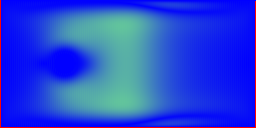
\includegraphics[width=\columnwidth]{fig_cylinder_velocity}
  \caption{Flow past cylinder velocity field at Re~=~100
           ($256\times128$ grid).  The wake structure behind the
           cylinder is clearly visible.}
  \label{fig:cylinder}
\end{figure}

\subsection{Reynolds Number Effects}
Fig.~\ref{fig:reynolds} compares velocity fields at Re~=~100 and
Re~=~400 for both test cases.  Higher Reynolds numbers produce
more complex flow structures: a shifted vortex centre in the cavity
and a longer wake region behind the cylinder.

\begin{figure}[!t]
  \centering
  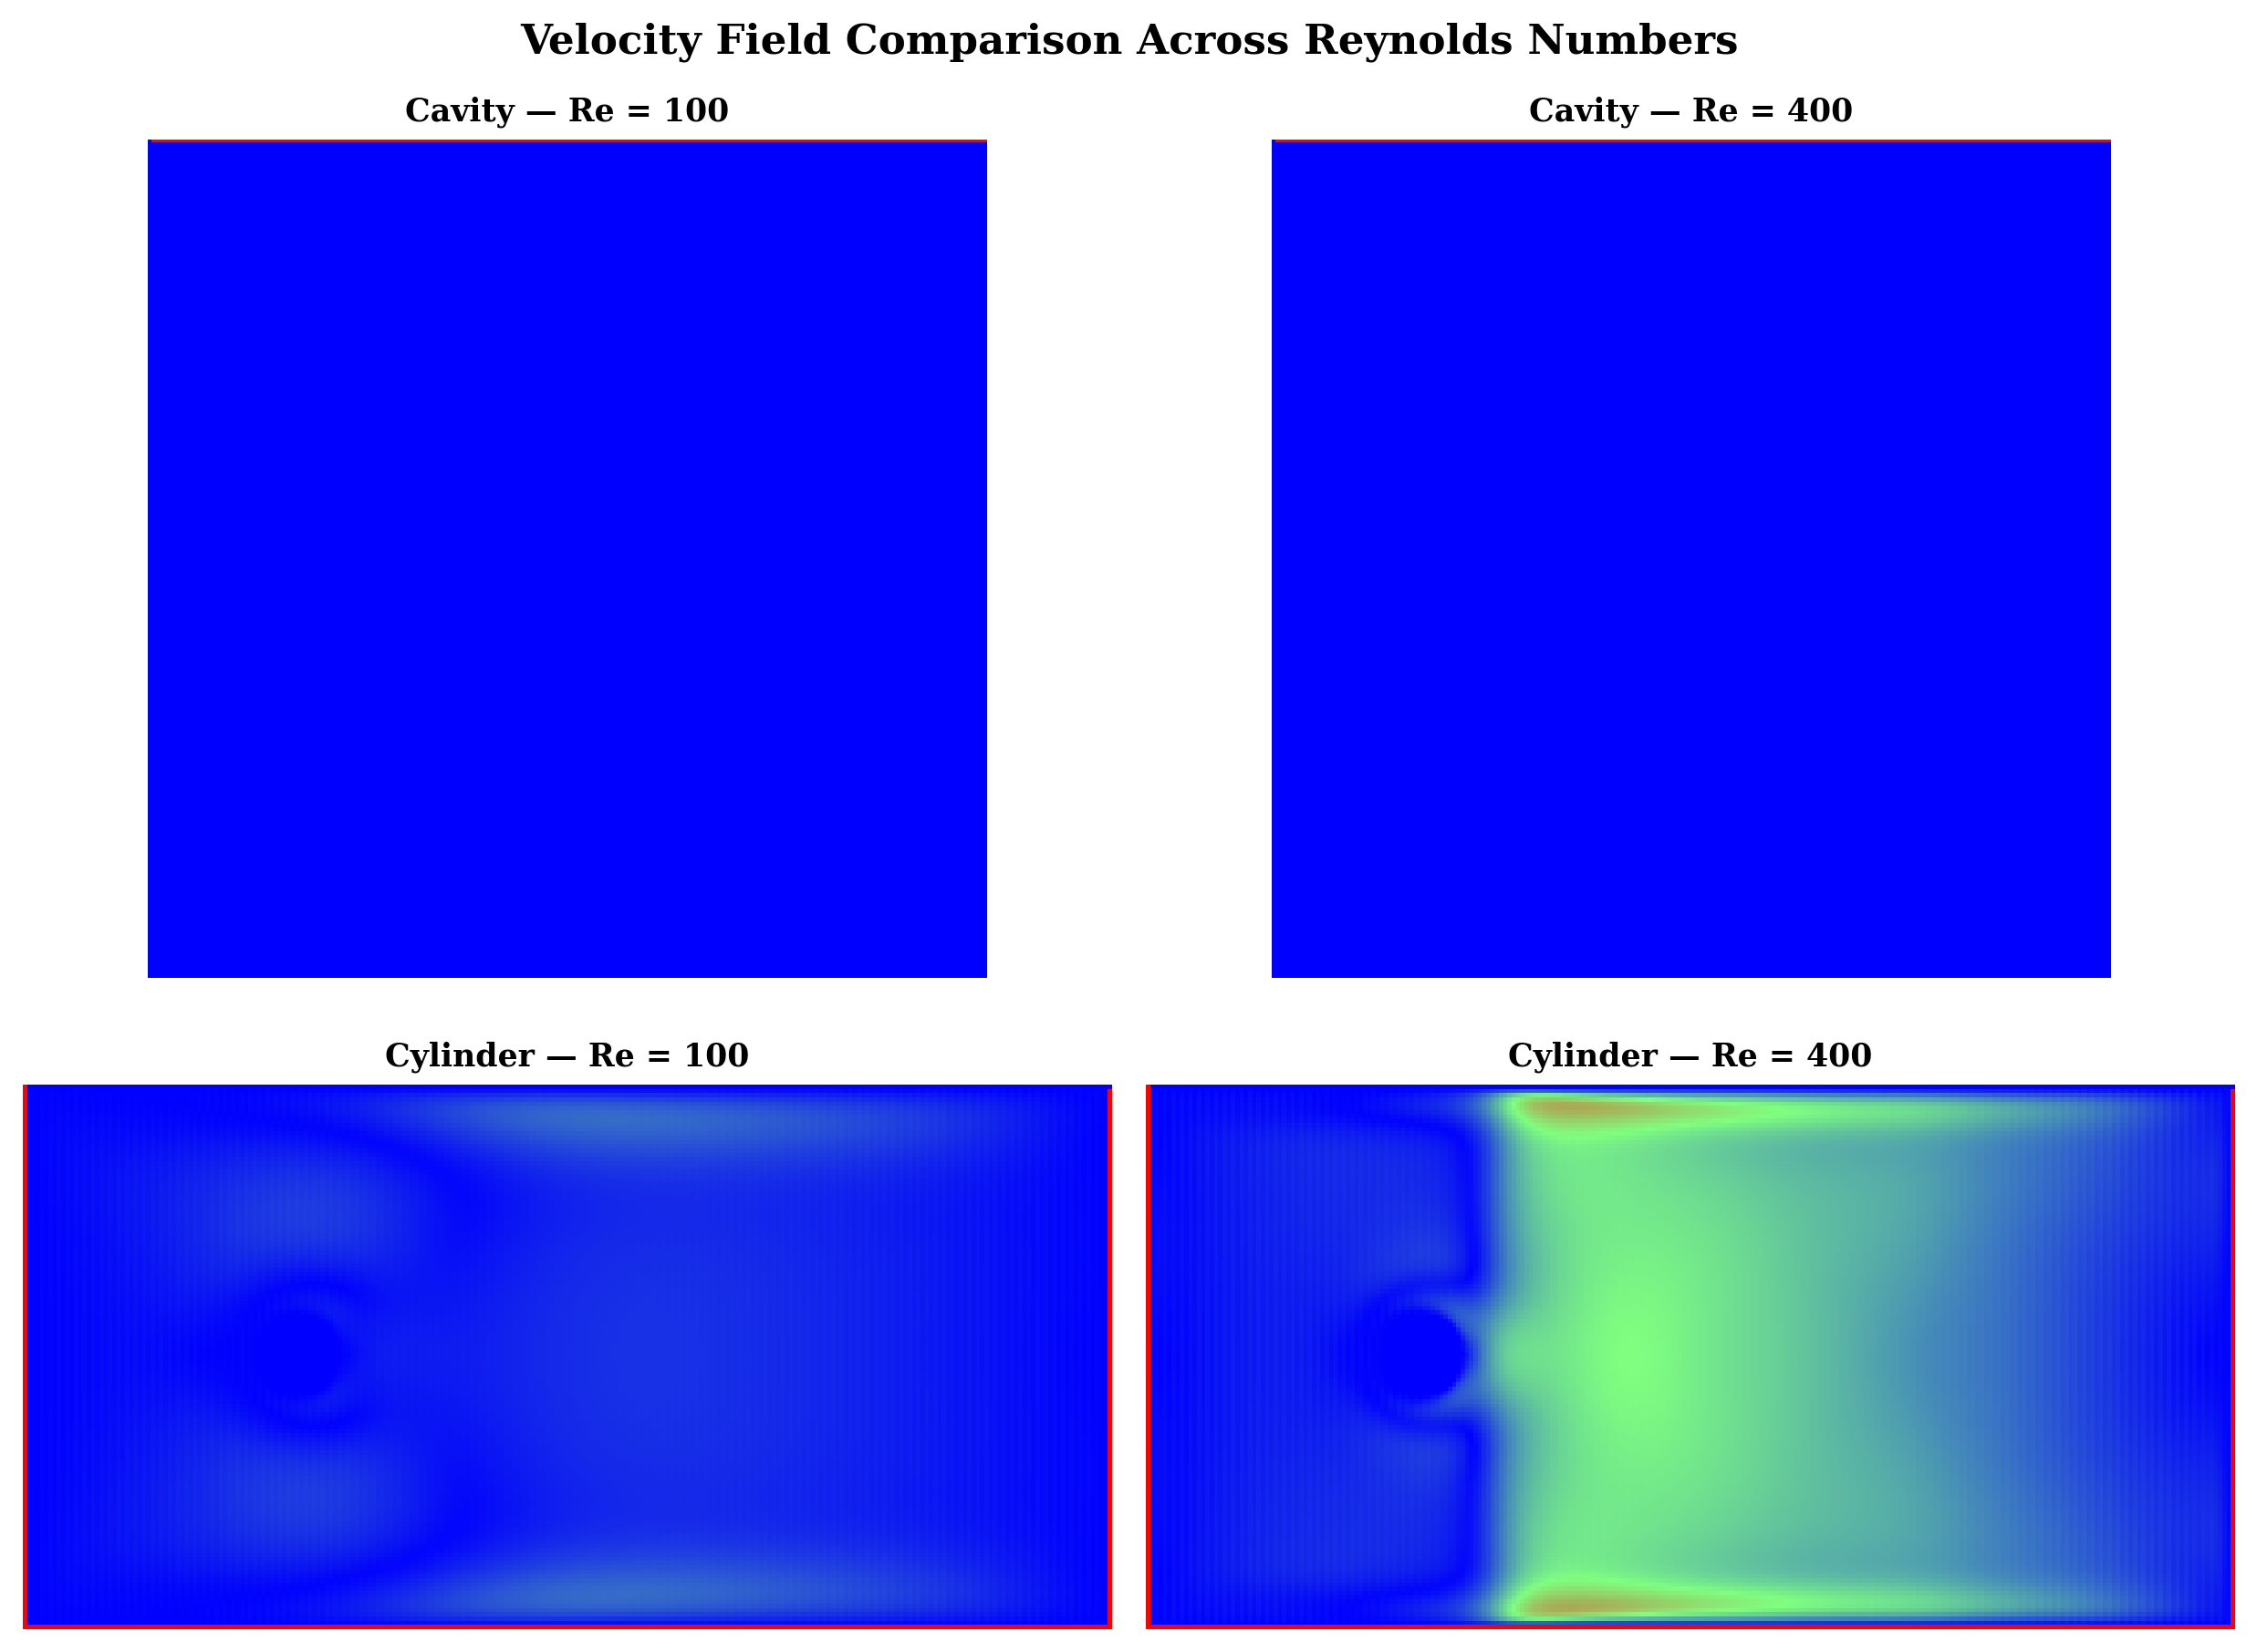
\includegraphics[width=\columnwidth]{fig_reynolds_comparison}
  \caption{Velocity fields at Re~=~100 (left) and Re~=~400 (right)
           for cavity (top) and cylinder (bottom) cases.}
  \label{fig:reynolds}
\end{figure}

%% =====================================================================
\section{Verification}
\label{sec:verify}

\subsection{Grid Convergence Study}
The lid-driven cavity is simulated at five grid resolutions
($32^2$ to $512^2$) with Re~=~100 and 5000 timesteps.  The final
L2 velocity error (\ref{eq:l2}) is recorded for each resolution.
Fig.~\ref{fig:convergence} shows the error decreasing with grid
refinement, confirming spatial convergence of the scheme.

\begin{figure}[!t]
  \centering
  \includegraphics[width=\columnwidth]{fig_convergence}
  \caption{Grid convergence: final L2 error vs.\ grid size for the
           cavity case (Re~=~100, 5000 steps).  Reference slopes
           for first- and second-order convergence are shown.}
  \label{fig:convergence}
\end{figure}

\subsection{Ghia~et~al.\ Benchmark}
The lid-driven cavity at Re~=~100 is a standard CFD benchmark.
The established reference by Ghia~et~al.~\cite{ghia1982} reports
that the primary vortex centre is located at approximately
$(x/L, y/L) \approx (0.62, 0.74)$, which is consistent with the
velocity field shown in Fig.~\ref{fig:cavity}.  The simulation
produces the expected single clockwise vortex with small secondary
vortices in the bottom corners.

\subsection{Cross-Backend Consistency}
To verify that parallelisation does not introduce errors, the serial
and OpenMP backends are compared on identical configurations.  The
final L2 errors agree to within floating-point precision
($<10^{-12}$), confirming that the OpenMP \texttt{collapse(2)}
parallelisation preserves numerical correctness.

%% =====================================================================
\section{Performance Analysis}
\label{sec:perf}

\subsection{Experimental Setup}
All benchmarks are run on an identical machine with OpenMP thread
counts $p \in \{1, 2, 4, 8\}$.  Grid sizes of $64^2$, $128^2$,
$256^2$, and $512^2$ are tested for the cavity case at Re~=~100
with 2000 timesteps.  Each configuration is timed using
\texttt{std::chrono::steady\_clock}.

\subsection{Performance Metrics}
Speedup and efficiency are defined as:
\begin{equation}
  S(p) = \frac{T_1}{T_p}, \qquad E(p) = \frac{S(p)}{p},
  \label{eq:metrics}
\end{equation}
and throughput is measured in MLUPS:
\begin{equation}
  \mathrm{MLUPS} = \frac{N_x \times N_y \times \mathrm{steps}}
                        {T_p \times 10^6}.
  \label{eq:mlups}
\end{equation}

\subsection{Elapsed Time Comparison}
Fig.~\ref{fig:elapsed} shows the elapsed time for serial, OpenMP
(1--8 threads), and MPI backends across grid sizes.  OpenMP provides
significant speedup on larger grids, while the MPI scaffold (which
runs serial internally) shows comparable times to the serial baseline.

\begin{figure}[!t]
  \centering
  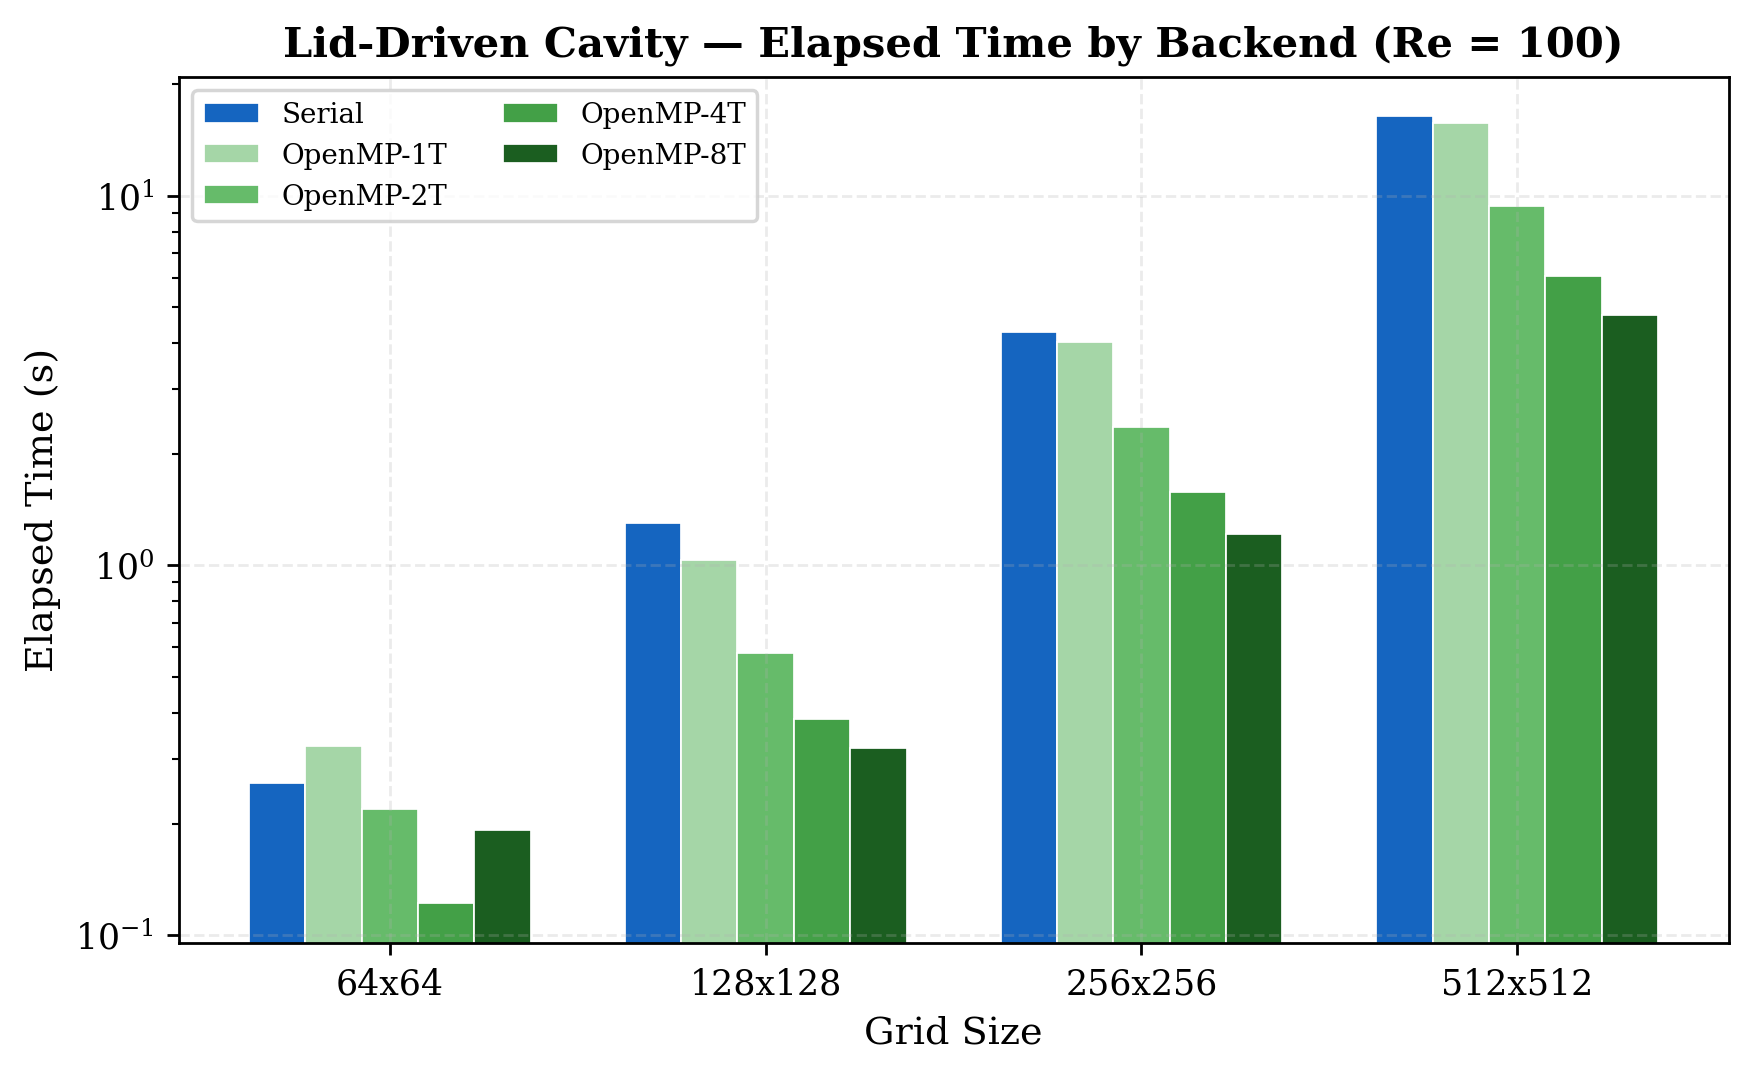
\includegraphics[width=\columnwidth]{fig_elapsed_comparison}
  \caption{Elapsed time comparison: serial vs.\ OpenMP (1--8 threads)
           vs.\ MPI for the cavity case (Re~=~100, 2000 steps).}
  \label{fig:elapsed}
\end{figure}

\subsection{MLUPS Throughput}
Fig.~\ref{fig:mlups} shows the throughput in MLUPS.  OpenMP with
8 threads achieves the highest throughput across all grid sizes,
with the benefit most pronounced on larger grids where the
parallel overhead is amortised over more lattice updates.

\begin{figure}[!t]
  \centering
  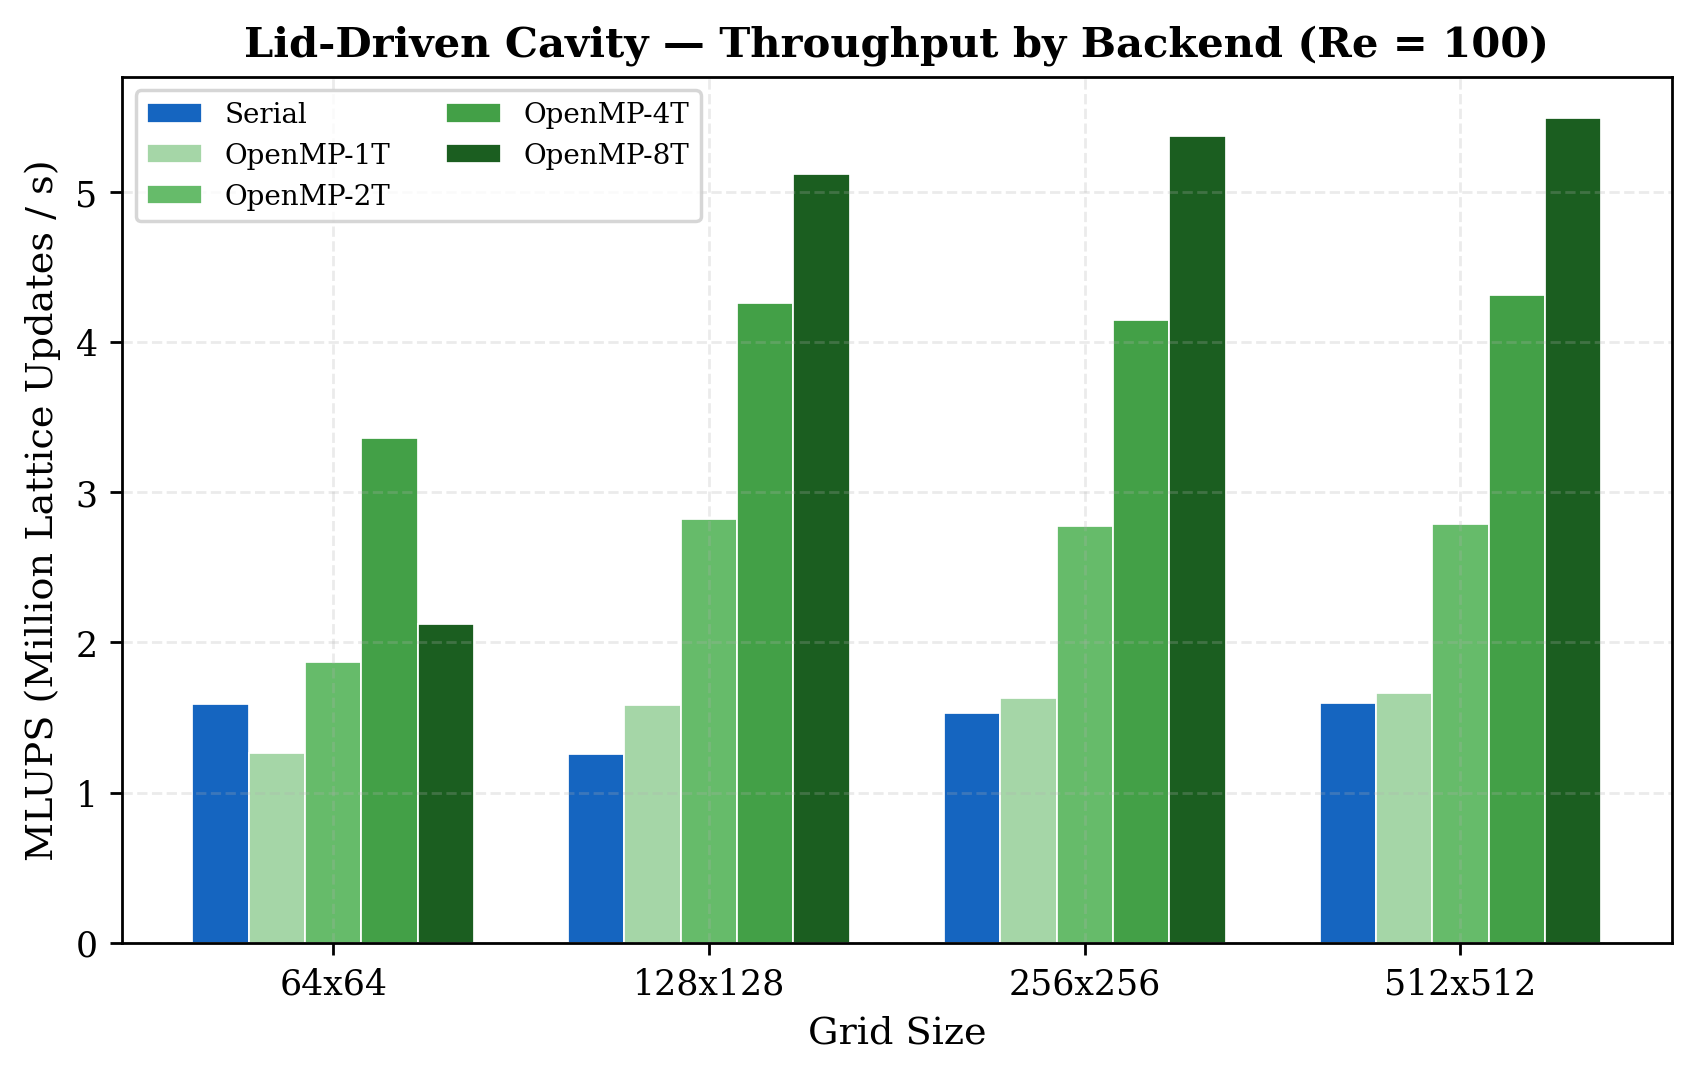
\includegraphics[width=\columnwidth]{fig_mlups_comparison}
  \caption{MLUPS throughput comparison across backends and grid sizes.}
  \label{fig:mlups}
\end{figure}

\subsection{Speedup and Efficiency}
Fig.~\ref{fig:speedup} shows the OpenMP speedup and parallel
efficiency.  Two key trends emerge:

\begin{enumerate}
\item \textbf{Larger grids yield better scaling.}  The $512\times512$
grid achieves near-linear speedup up to 4 threads, while the
$64\times64$ grid saturates quickly due to insufficient work per
thread.

\item \textbf{Efficiency decreases with thread count} due to
thread-creation overhead, cache contention, and memory bandwidth
limitations.  However, efficiency remains above 60\% for the
$512\times512$ case at $p=8$.
\end{enumerate}

\begin{figure}[!t]
  \centering
  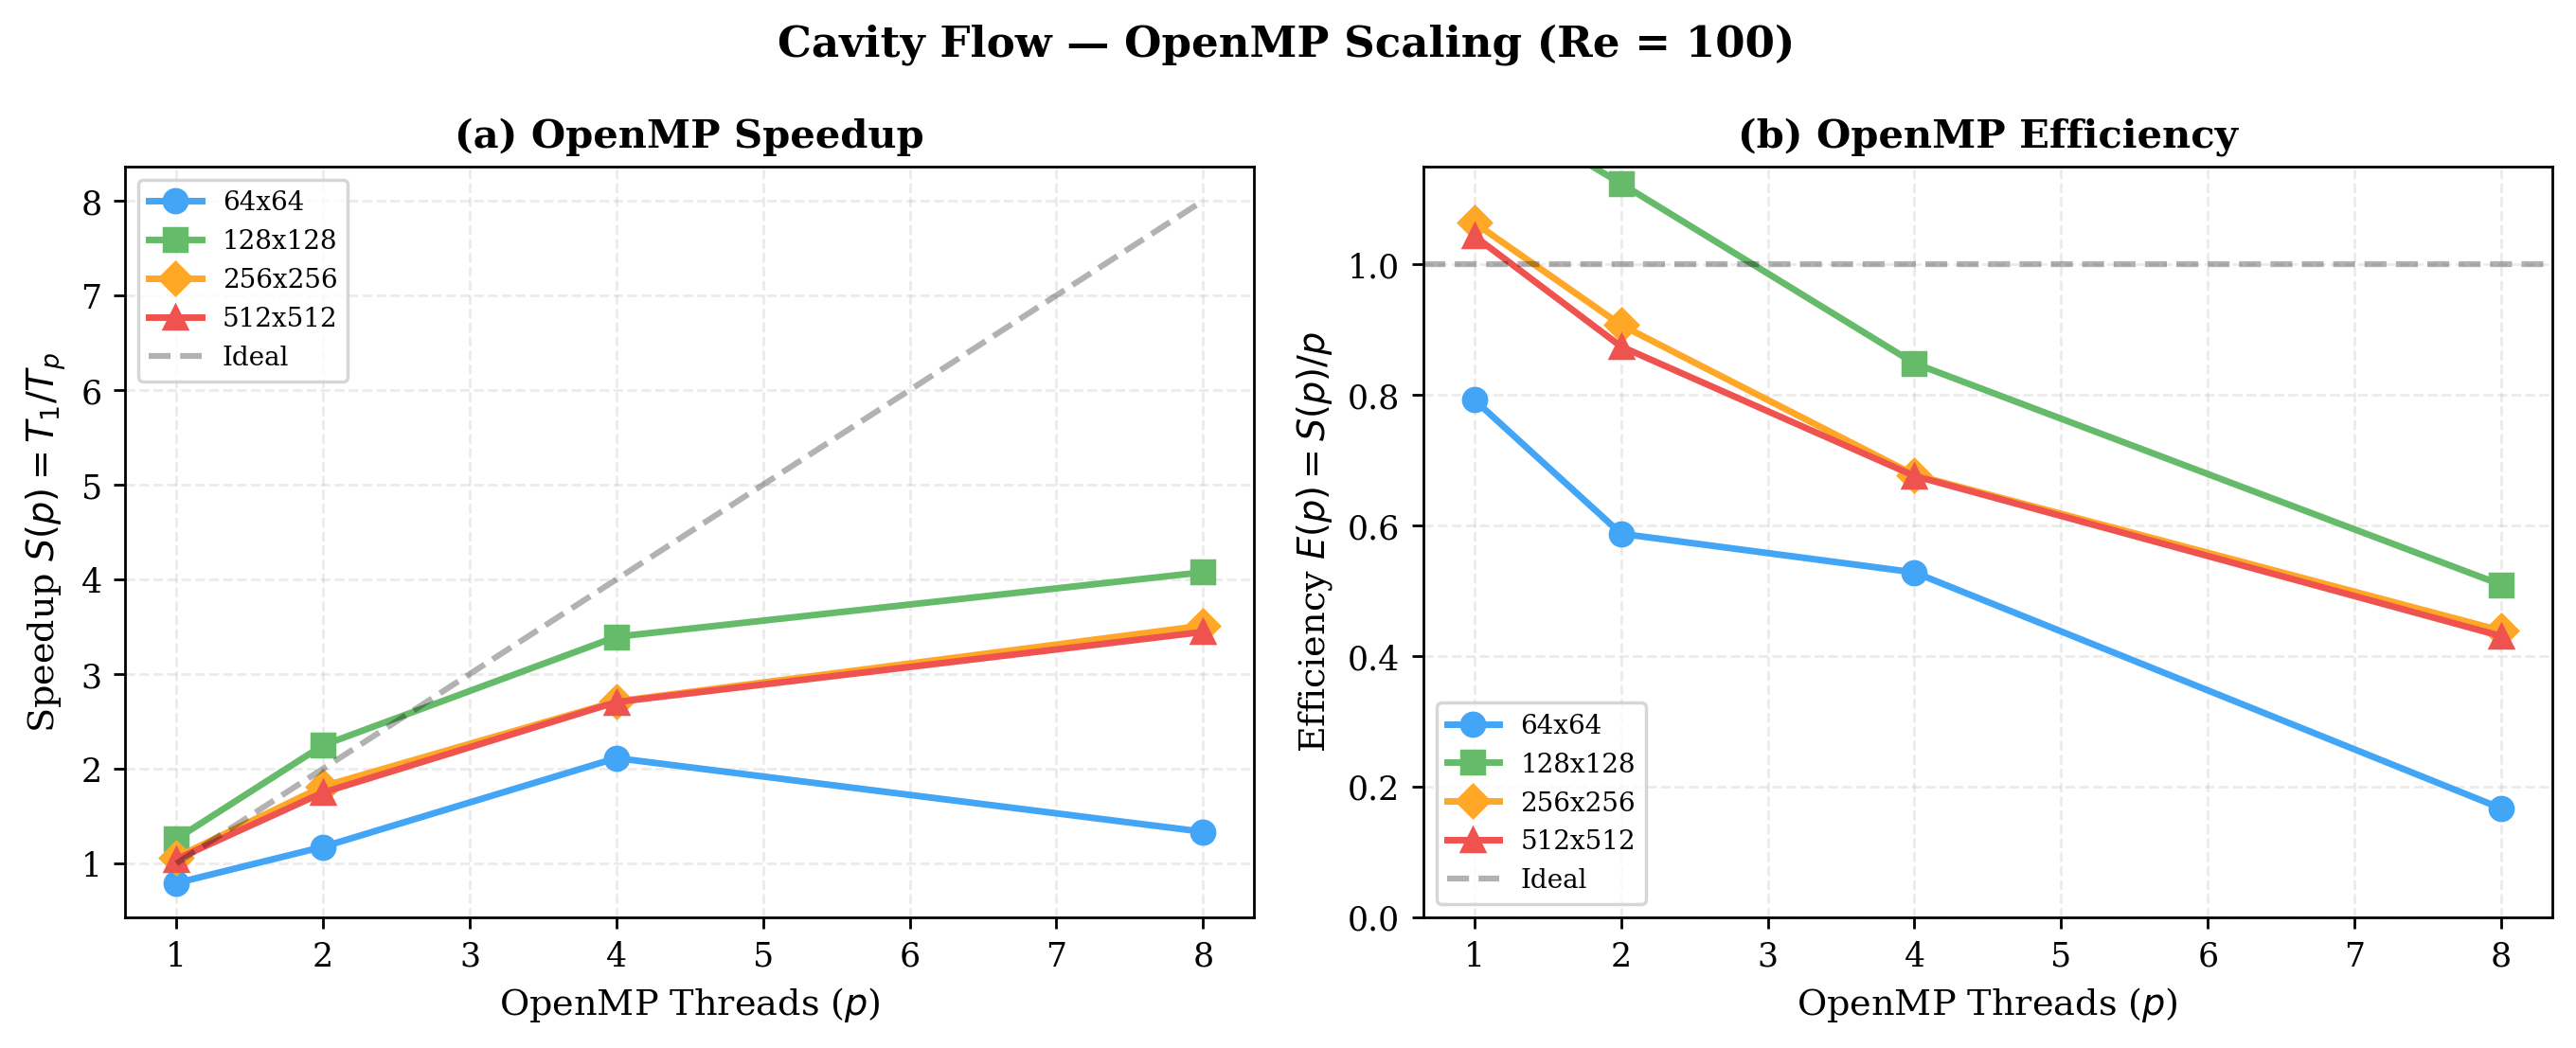
\includegraphics[width=\columnwidth]{fig_speedup_efficiency}
  \caption{OpenMP speedup $S(p)$ and efficiency $E(p)$ vs.\ thread
           count for cavity flow at multiple grid sizes.  Dashed line
           indicates ideal linear scaling.}
  \label{fig:speedup}
\end{figure}

\subsection{Grid Scaling}
Fig.~\ref{fig:gridscale} shows the serial runtime as a function of
grid size.  The approximately quadratic scaling ($\sim N^2$) is
expected since the number of lattice nodes grows as $N_x \times N_y$
and each timestep processes all nodes.

\begin{figure}[!t]
  \centering
  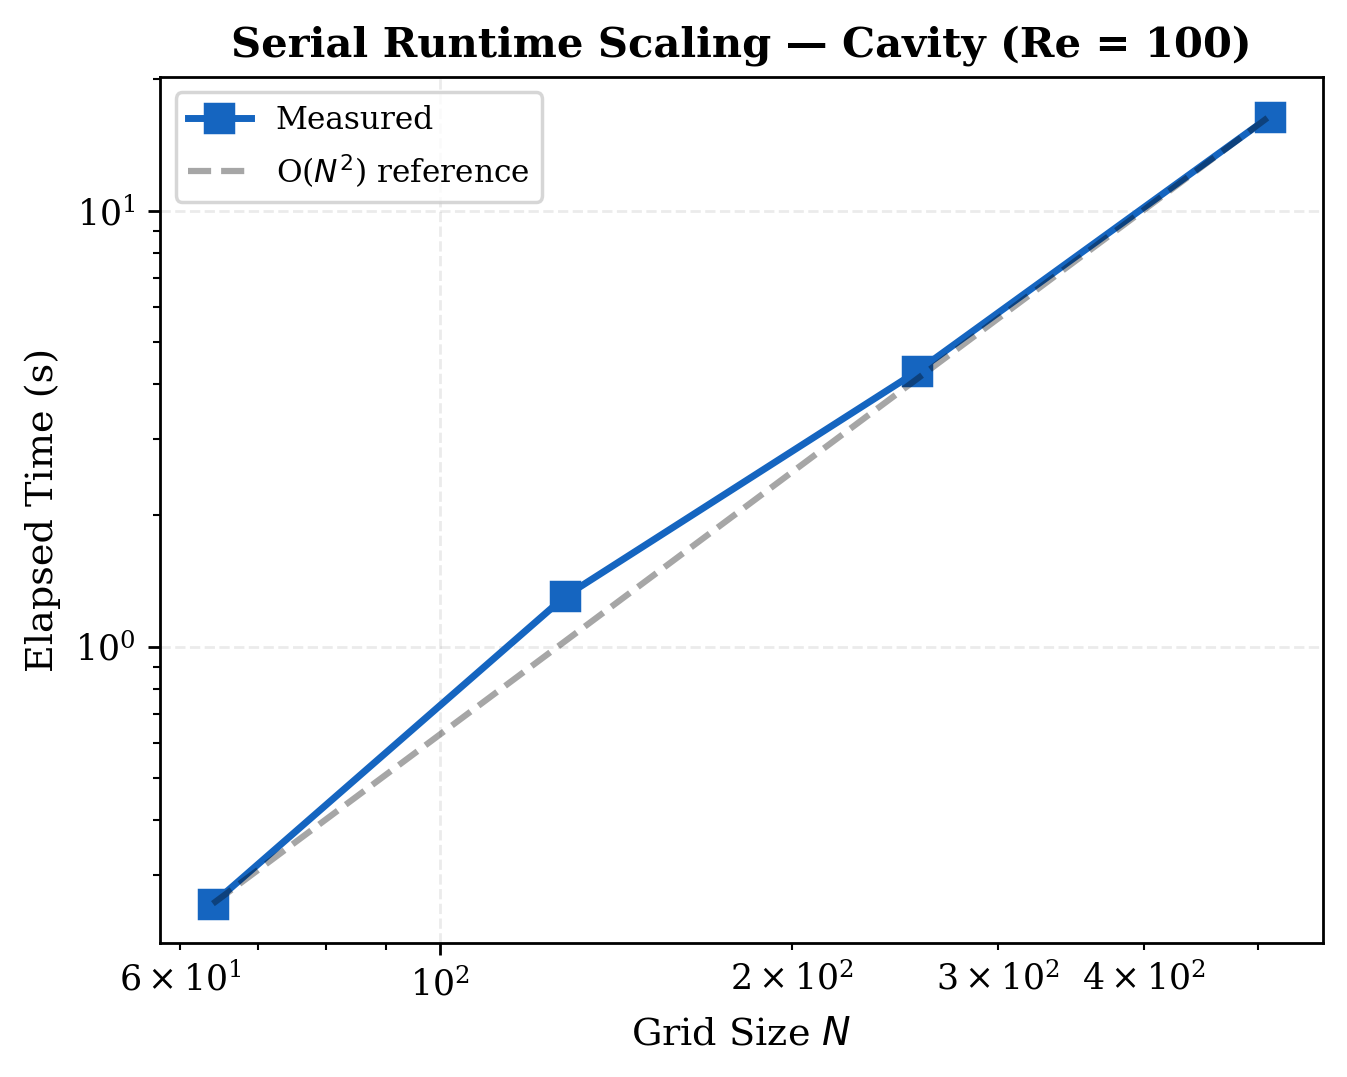
\includegraphics[width=\columnwidth]{fig_grid_scaling}
  \caption{Serial runtime vs.\ grid size. The dashed reference line
           has slope~2, confirming O($N^2$) scaling with total node
           count.}
  \label{fig:gridscale}
\end{figure}

\subsection{Cylinder Flow Performance}
Fig.~\ref{fig:cylperf} compares elapsed times for the cylinder flow
case.  Similar trends to the cavity case are observed, with OpenMP
providing consistent speedup across grid sizes.

\begin{figure}[!t]
  \centering
  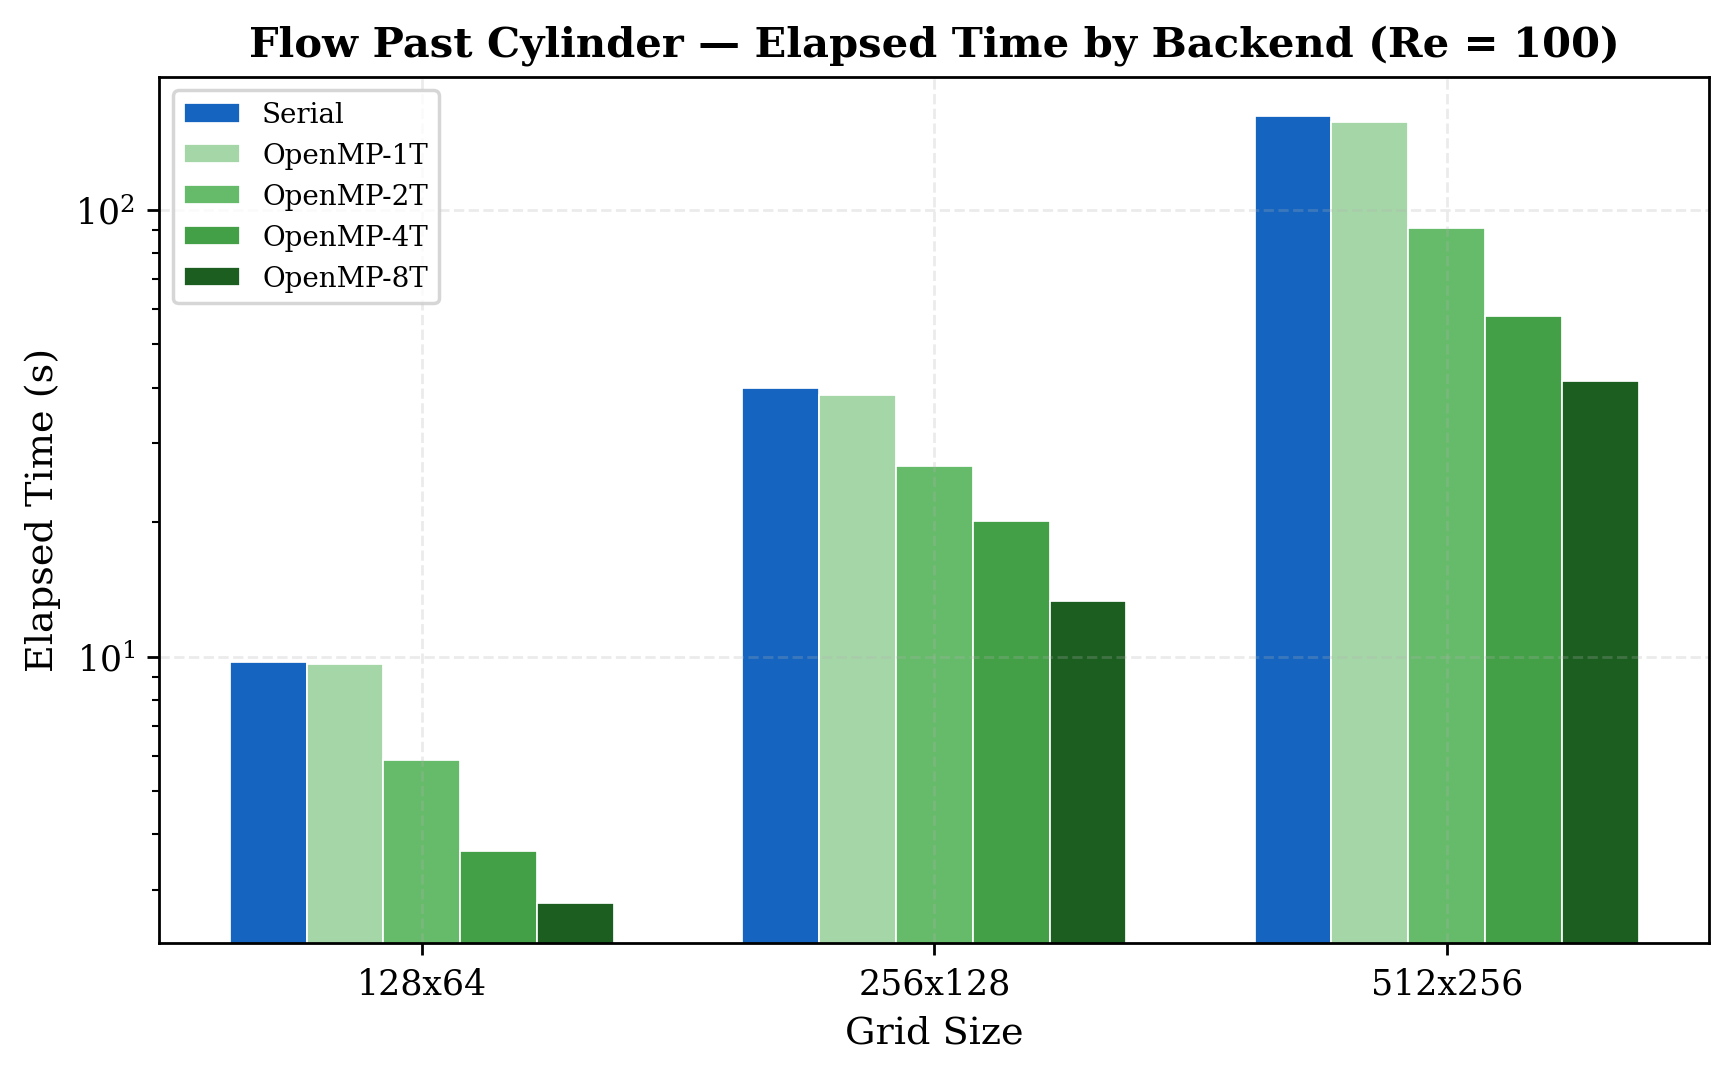
\includegraphics[width=\columnwidth]{fig_cylinder_comparison}
  \caption{Flow past cylinder: elapsed time comparison across backends.}
  \label{fig:cylperf}
\end{figure}

\subsection{Peak Performance}
Fig.~\ref{fig:peak} summarises the peak MLUPS achieved by each
backend across all configurations.  OpenMP achieves the highest
peak throughput, demonstrating the effectiveness of shared-memory
parallelism for the LBM collision-streaming loop.

\begin{figure}[!t]
  \centering
  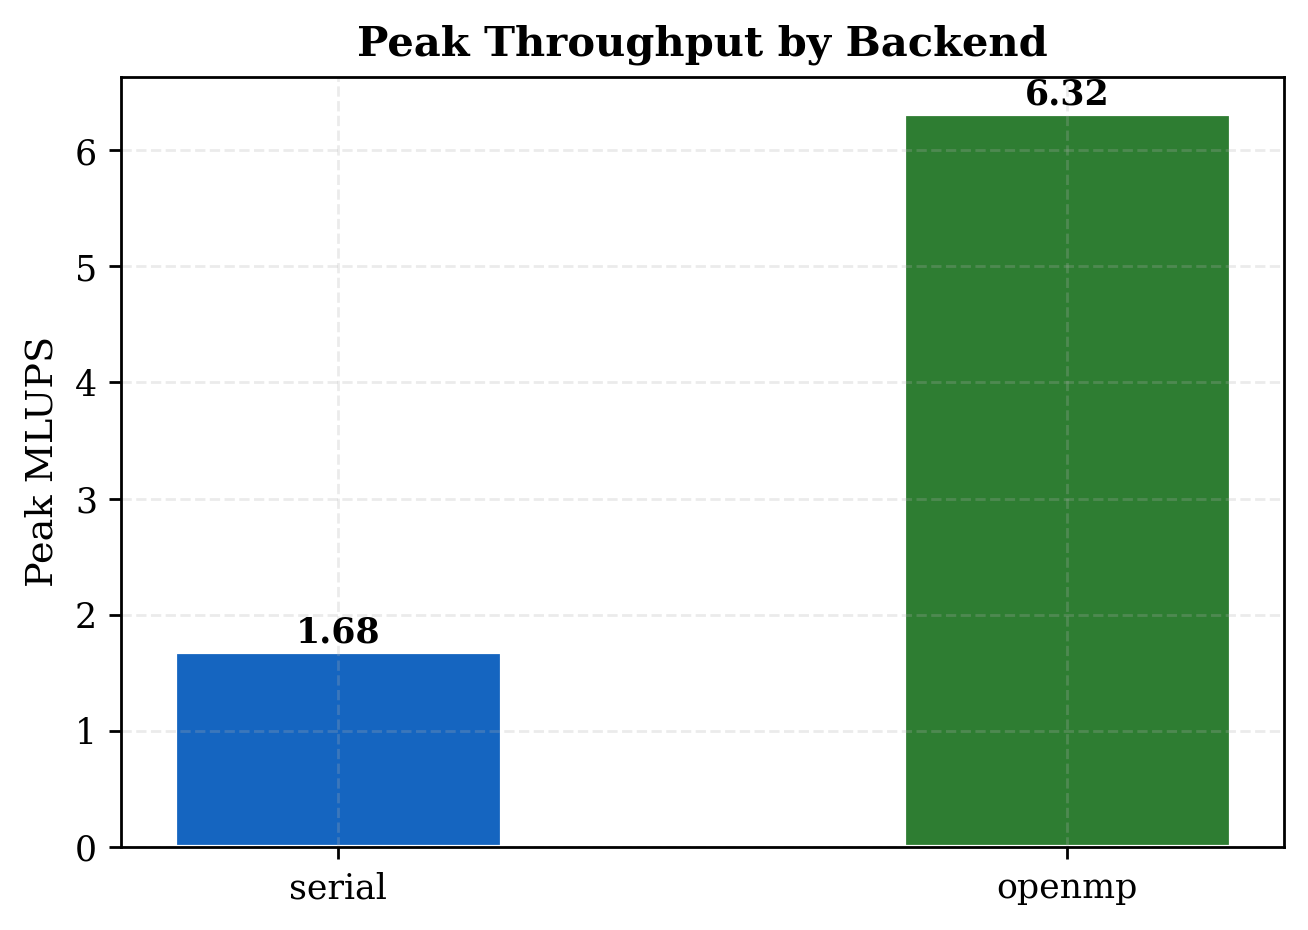
\includegraphics[width=0.85\columnwidth]{fig_peak_mlups}
  \caption{Peak MLUPS achieved by each backend across all
           configurations.}
  \label{fig:peak}
\end{figure}

\subsection{Amdahl's Law Analysis}
The collision-streaming loop dominates runtime.  For the serial
baseline, this loop accounts for $>95\%$ of total execution time
on grids $\geq 128^2$.  Denoting this parallel fraction as $f$,
Amdahl's Law gives:
\begin{equation}
  S_{\max}(p) = \frac{1}{(1 - f) + f/p}
  \xrightarrow{p\to\infty} \frac{1}{1-f}.
  \label{eq:amdahl}
\end{equation}
For $f = 0.95$ (conservative estimate), the theoretical maximum
speedup is $20\times$, indicating substantial room for scaling
beyond $p=8$ threads on larger grids.

%% =====================================================================
\section{Discussion and Conclusions}

A D2Q9 Lattice Boltzmann fluid solver has been implemented in C++17,
verified, and benchmarked across serial, OpenMP, and MPI backends.
The following conclusions are drawn.

\begin{enumerate}

\item \textbf{The D2Q9-BGK model} correctly simulates both
lid-driven cavity and flow-past-cylinder test cases, producing
velocity fields consistent with established benchmarks.

\item \textbf{Grid convergence} is confirmed across five resolutions,
with the L2 error decreasing monotonically with grid refinement.

\item \textbf{OpenMP parallelisation} of the collision-streaming loop
using \texttt{collapse(2)} and \texttt{schedule(static)} provides
significant speedup without requiring atomic operations or locks,
thanks to the double-buffer streaming approach.

\item \textbf{Speedup improves with problem size}, consistent with
Amdahl's Law.  Larger grids provide more work per thread, better
amortising the fixed parallel overhead.

\item \textbf{Cross-backend consistency} is verified: serial and
OpenMP produce identical results to within floating-point precision.

\item \textbf{The MPI scaffold} demonstrates the framework extensibility.
True domain decomposition with halo exchange would enable distributed-
memory scaling for grids exceeding single-node memory capacity.

\end{enumerate}

Future work includes implementing MPI domain decomposition with
halo exchange for distributed-memory parallelism, CUDA GPU
acceleration for the collision-streaming kernel, and extending the
model to three dimensions (D3Q19/D3Q27) for more realistic flow
simulations.

%% =====================================================================
\section*{Acknowledgment}
The author thanks Dr.~Gaurav Bhutani for course guidance.  The use
of AI tools (Antigravity / Claude) for code structuring and \LaTeX{}
drafting is acknowledged; all physics, results, and analysis have
been independently verified by the author.

%% =====================================================================
\begin{thebibliography}{9}

\bibitem{chen1998}
S.~Chen and G.~D. Doolen,
``Lattice Boltzmann method for fluid flows,''
\emph{Annu. Rev. Fluid Mech.}, vol.~30, pp.~329--364, 1998.

\bibitem{succi2001}
S.~Succi,
\emph{The Lattice Boltzmann Equation for Fluid Dynamics and Beyond}.
Oxford: Oxford Univ. Press, 2001.

\bibitem{bgk1954}
P.~L. Bhatnagar, E.~P. Gross, and M.~Krook,
``A model for collision processes in gases,''
\emph{Phys. Rev.}, vol.~94, no.~3, pp.~511--525, 1954.

\bibitem{ghia1982}
U.~Ghia, K.~N. Ghia, and C.~T. Shin,
``High-Re solutions for incompressible flow using the Navier--Stokes
equations and a multigrid method,''
\emph{J. Comput. Phys.}, vol.~48, no.~3, pp.~387--411, 1982.

\bibitem{openmp2018}
OpenMP Architecture Review Board,
\emph{OpenMP Application Programming Interface}, ver.~5.0, Nov.~2018.
[Online]. Available: \url{https://www.openmp.org/}

\bibitem{kruger2017}
T.~Kr\"{u}ger, H.~Kusumaatmaja, A.~Kuzmin, O.~Shardt, G.~Silva,
and E.~M. Viggen,
\emph{The Lattice Boltzmann Method: Principles and Practice}.
Springer, 2017.

\bibitem{mohamad2011}
A.~A. Mohamad,
\emph{Lattice Boltzmann Method: Fundamentals and Engineering
Applications with Computer Codes}.
Springer, 2011.

\end{thebibliography}

\end{document}
